\documentclass[UTF8]{ctexart}
\usepackage{booktabs}  % professionally typeset tables
\usepackage{amsmath}
\usepackage{setspace}
\usepackage{textcomp}  % better copyright sign, among other things
\usepackage{xcolor}
\usepackage{lipsum}    % filler text
\usepackage{subfig}   
\usepackage{geometry}
\usepackage{float}
\usepackage{hyperref}
\usepackage{graphicx}


\geometry{left=2.54cm,right=2.54cm,top=2.18cm,bottom=3.18cm}
\date{}
\title{\textbf{竞赛讲座管理系统设计文档}}
\author{\rightline{SigmaGo小组}} 


\begin{document}
%\begin{CJK}{UTF8}{gbsn}
\begin{spacing}{1.3}
\maketitle


\section{简介}
\subsection{系统简介}
系统收集讲座、竞赛组织方的组织的讲座信息,同时根据用户的信息进行竞赛、讲座内容的推荐。

\subsection{系统定位}
针对于校园中讲座和竞赛资源的流通性不足、同学们获取信息和资源的方式过于分散等问题,我们小组希望能够设计一个竞赛讲座管理系统,通过对于竞赛、讲座等信息进行统一整理和总结,并且设计一种算法对于特定同学进行合适的讲座和竞赛的推荐,增加同学们对于自己所需要的讲座、感兴趣的竞赛的认知,从而实现信息的最大化利用。



\subsection{系统功能}
\begin{itemize}
    \item 实现用户的注册和登录,对于用户的个人信息进行采集;
    
    \item 实现针对于用户的个人兴趣爱好等,进行特定竞赛讲座推荐;
    
    \item 实现讲座、竞赛管理方对于讲座和竞赛信息的录入;
    
    \item 实现管理员对于竞赛、讲座的管理;
    
    \item 实现简单的讲座、竞赛搜索功能。
\end{itemize}


\subsection{目标用户}
校内对于竞赛、讲座感兴趣的学生以及校园内各种竞赛、讲座的管理人员。

\subsection{运行环境}
运行在网页和微信平台上,分为前端和后端,整体通过Django进行整体框架的管理。作为真个框架的最重要的核心部分,我们采用的是Django框架。 Django是一个开放源代码的Web应用框架,由Python写成。 Django遵守BSD版权,初次发布于2005年7月, 并于2008年9月发布了第一个正式版本1.0 。Django采用了MVC的软件设计模式,即模型M,视图V和控制器C。

\section{系统框架(类图)}

\subsection{功能模块}
		\begin{figure}[H]
				\centering
				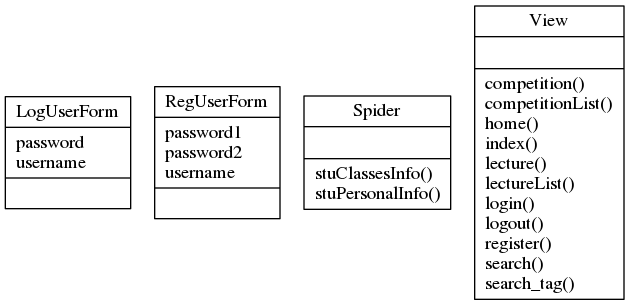
\includegraphics[width=\textwidth]{images//classes_view.png}
		\end{figure}

\subsection{数据库模块}
		\begin{figure}[H]
				\centering
				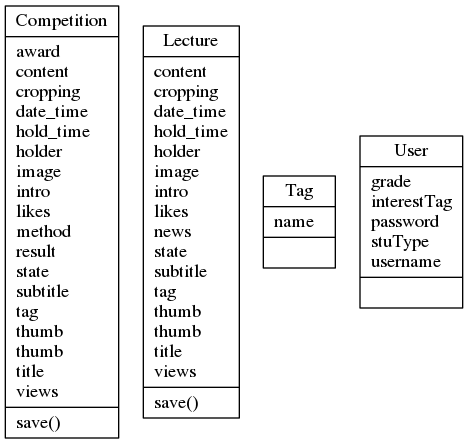
\includegraphics[width=\textwidth]{images//classes_model.png}
		\end{figure}
		
\section{UI设计}
\subsection{前端设计}
%%你可以假象一下这里有图233
\begin{figure}[h]
    \centering
    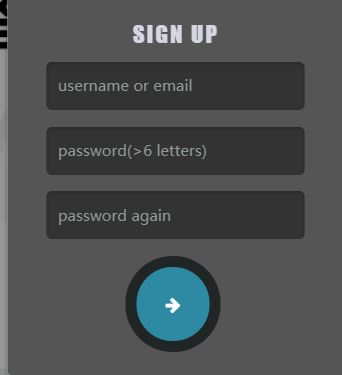
\includegraphics{images//signup.JPG}
    \caption{注册页面}
    \label{imgaes//fig:signup}
\end{figure}

\begin{figure}[h]
    \centering
    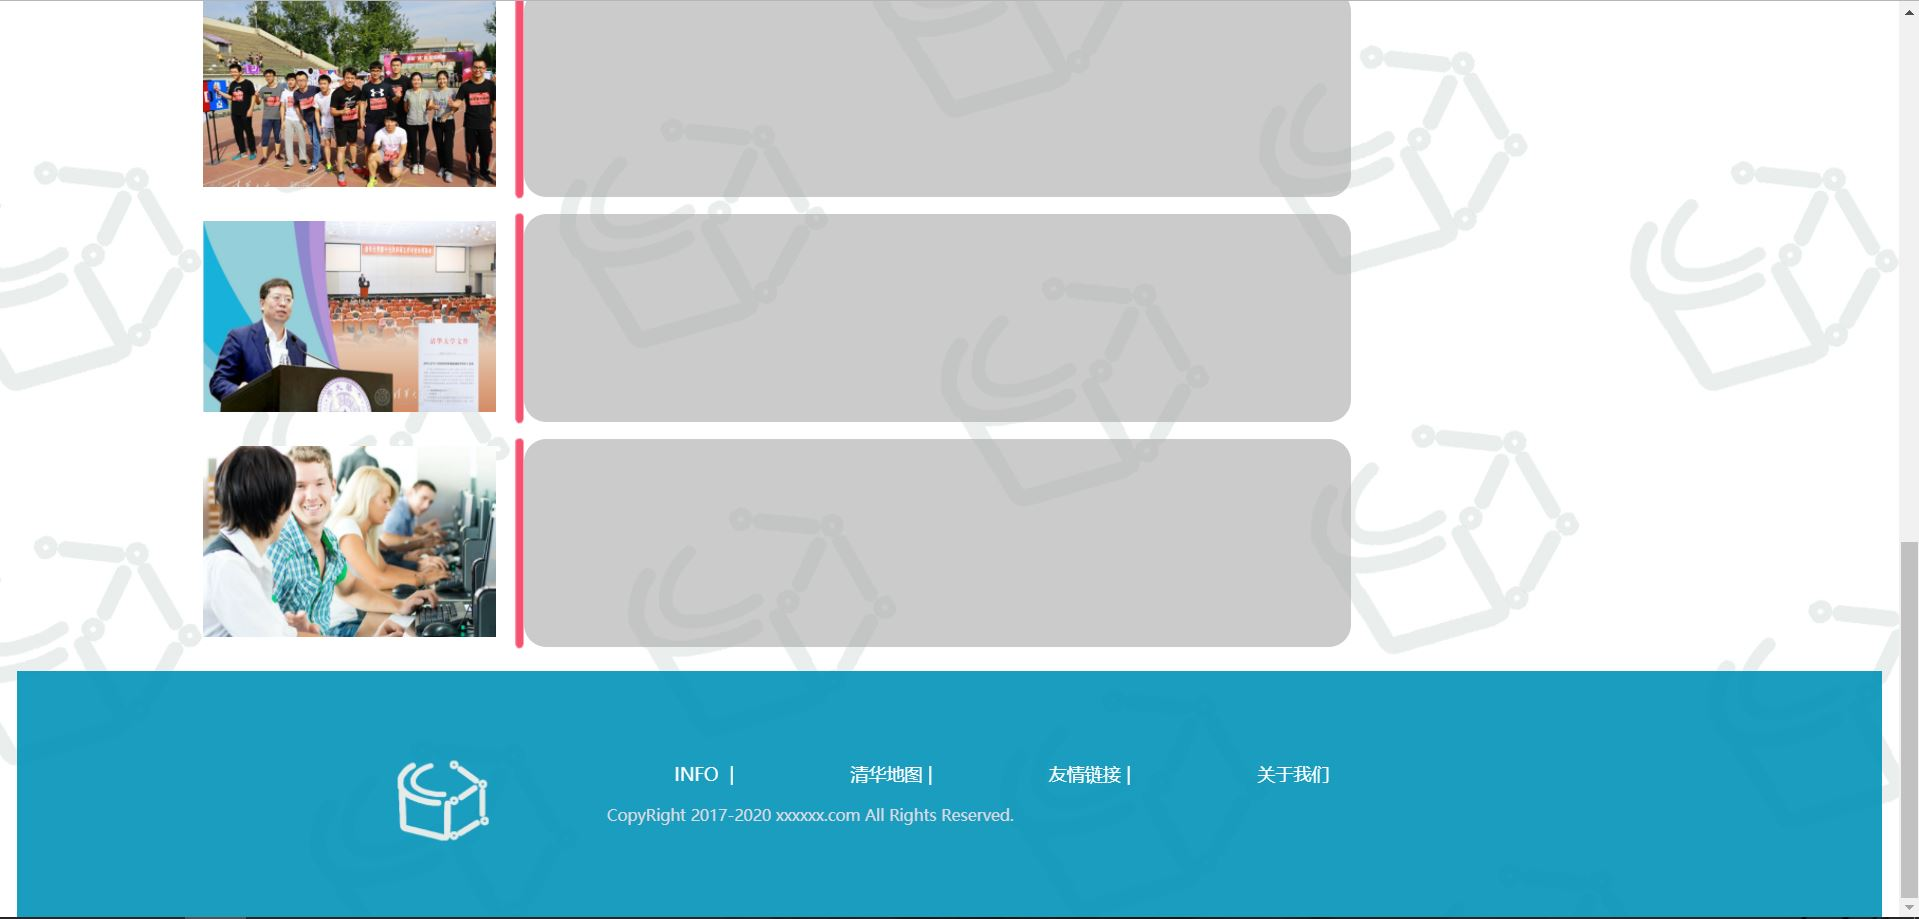
\includegraphics[width=\textwidth]{images//images.JPG}
    \caption{竞赛列表}
    \label{fig:competition}
\end{figure}

\begin{figure}[h]
    \centering
    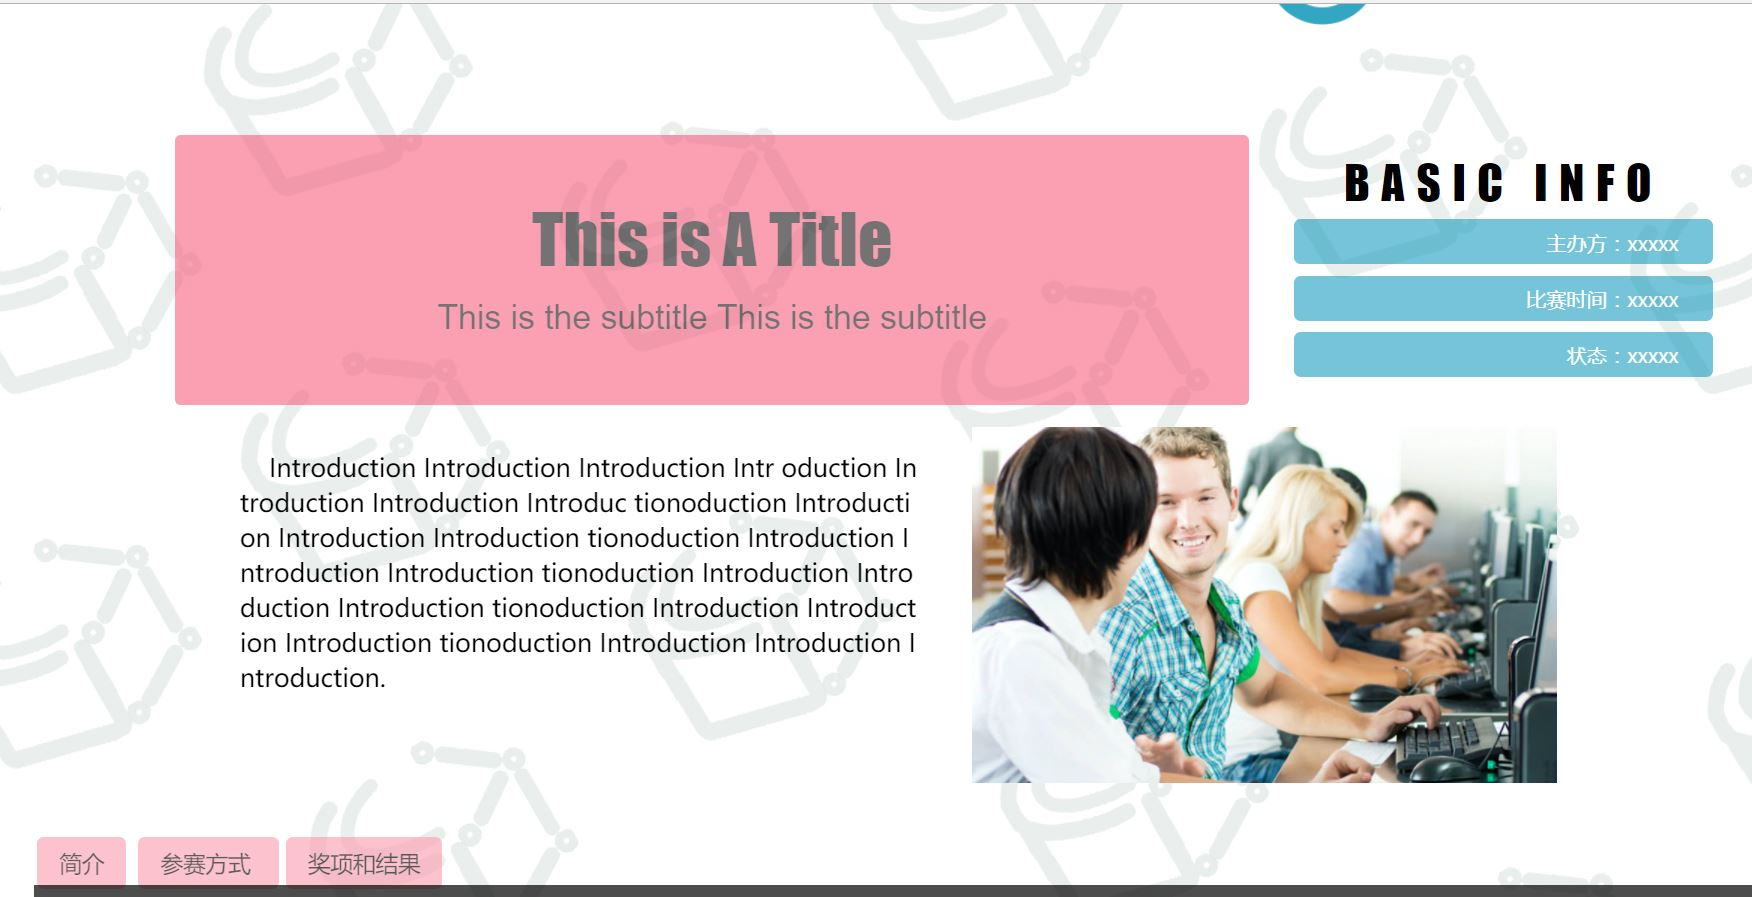
\includegraphics[width=\textwidth]{images//singleinfo.JPG}
    \caption{单个讲座页面}
    \label{fig:single}
\end{figure}

\begin{figure}[h]
    \centering
    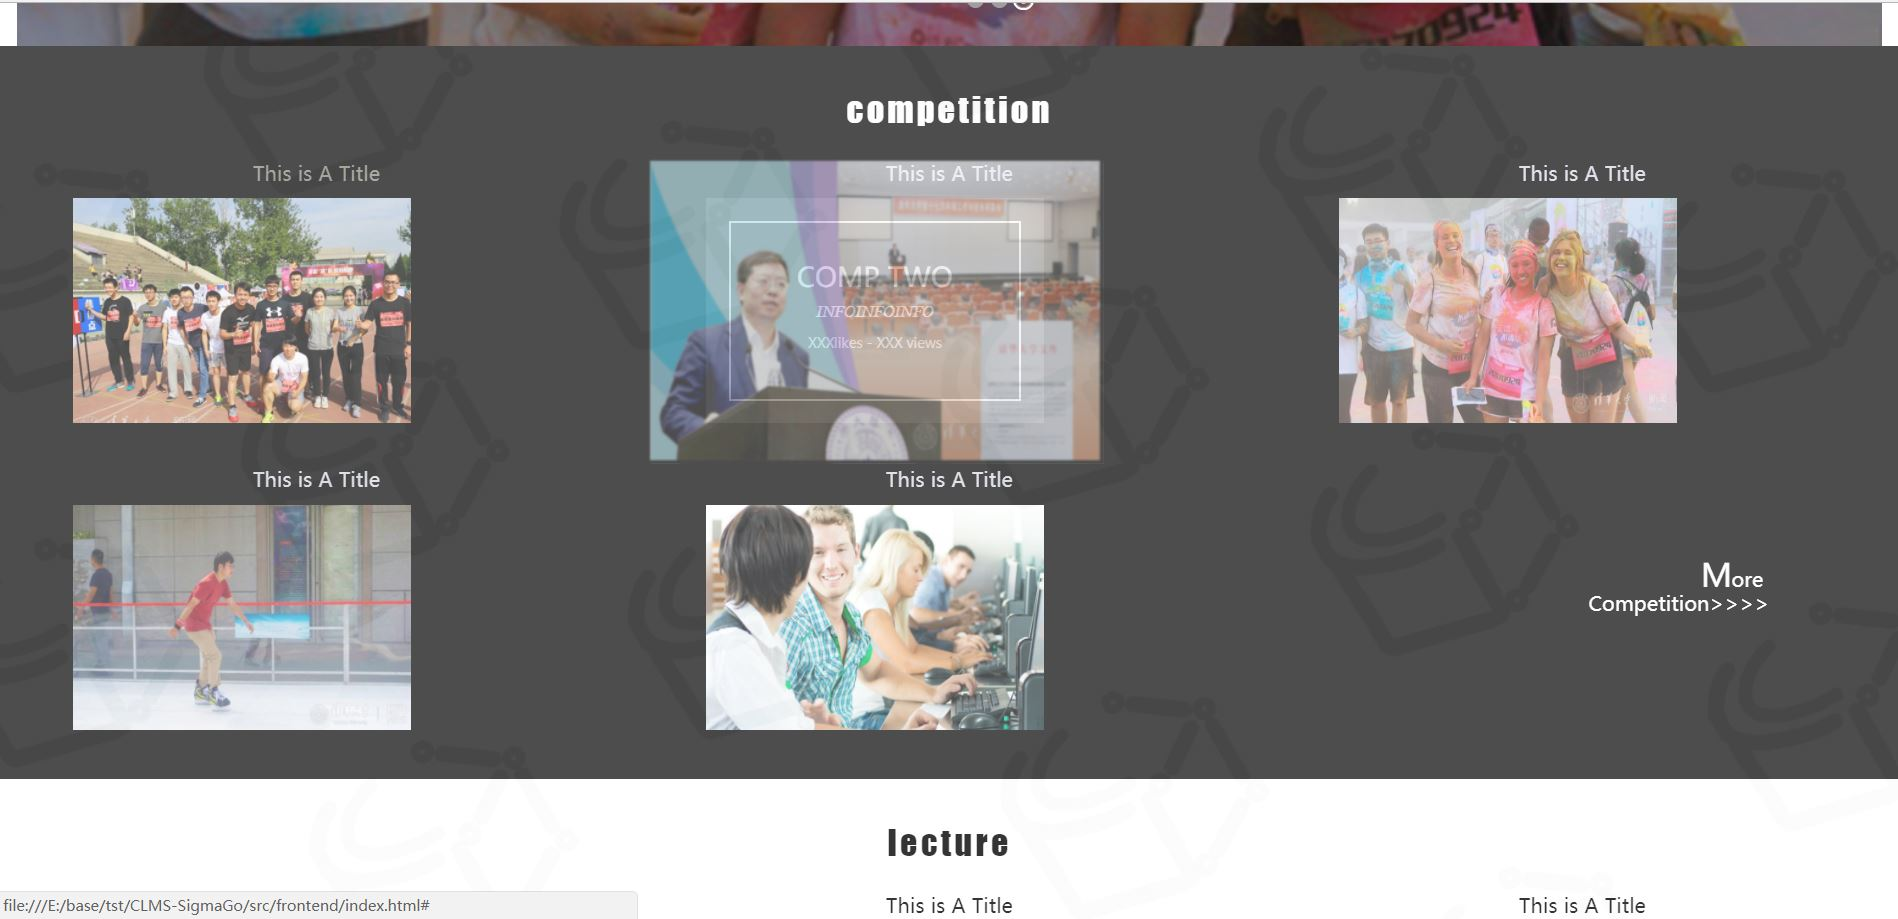
\includegraphics[width=\textwidth]{images//comptetition.JPG}
    \caption{讲座页面集合}
    \label{fig:collection}
\end{figure}

%\section{实验收获与小结}
%\section{程序来源说明}
\end{spacing}
\end{document}
